\section{Dataset}
Nordjyske is a Danish news agency that maintains multiple newspapers, radios, and other news sources throughout north Jutland, a region in Denmark.
They store their news articles in a non-public database, where each article contains multiple meta-data fields which describes some aspect of the data eg. author.
The dataset, we use, ranges from 2017 to 2019 and contains 139261 articles that use a vocabulary of 69192 unique words after preprocessing.
One of the meta-data fields is the Category field, which both describes where the article is supposed to be located(within a newspaper) and also which subject the article is about.

In the following section, we describe each of the meta-data fields which are analyzed.

\subsection{Author}
This field is for the author, who has written the article.
Each article only has a single author, so we do not account for multiple authors.
This field is fully observed within the dataset, which means that every article has one author.
There are $227$ different authors within the dataset.
%and they are almost evenly distributed in the number of articles they have written.

\subsection{Category}
% what it is?
The category field describes a variety of different aspects.
A proportion of the categories contains which specific newspaper, they belong to, eg. 'Aalborg-Newspaper'.
Another proportion of the category fields describes the overall subject of the document, such as 'Culture' and 'Sports-newspaper'.
% stats
This field is fully observed within the dataset and there are originally $58$ different categories in the dataset.
However, while most of these categories cover a significant number of documents, there are some categories which are only used by a few documents.

Filtering away all categories covering less than $140$ documents ($0.01\%$ of the total document set) and combining them into a single new 'misc' category, $34$ categories remain.
\autoref{fig:category_box} shows an overview of the size of the categories.\langballe[inline]{consider showing name of categories and relvative dataset size.}

\begin{figure}
	\centering
	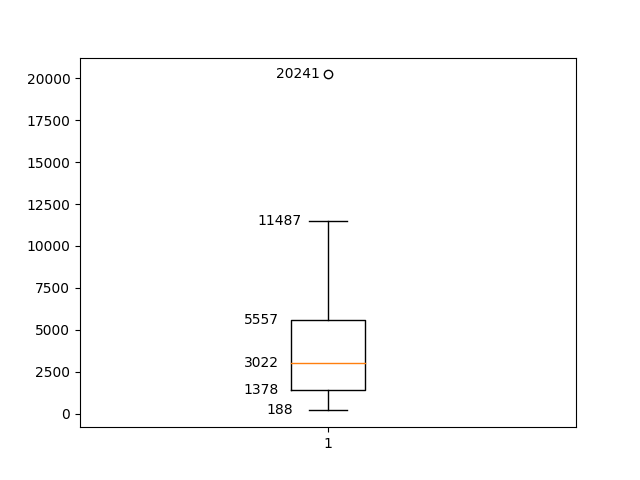
\includegraphics[width=1 \linewidth]{figures/category_box.png}
	\caption{Boxplot over the size of the categories. Size meaning the amount of documents with the same category.}
	\label{fig:category_box}
\end{figure}

\subsection{Taxonomy}
The taxonomy field describes a hierarchical structure of the topical or geographical subject of the articles.
This field is only partially observed within the dataset, which means that roughly $50\%$ of the articles contain this field.
We observe a general pattern when traversing this field which is:
\begin{itemize}
	\item Places/Country/Region/Town
	\item Topics/Sub-Topic/Subsub-topic
\end{itemize}
Examples of this field are:
\begin{itemize}
	\item PLACES/Danmark/Nordjylland/Aalborg/Lillevorde
	\item TOPICS/Religion/Christianity
\end{itemize}
About $80\%$ of the observed variables contain the Places variable and $20\%$ is using the topics variable. 

